\documentclass[tikz,border=8pt]{standalone}
\usepackage[T1]{fontenc}
\usepackage{lmodern}
\renewcommand{\familydefault}{\sfdefault}
\usepackage{tikz}
\usetikzlibrary{arrows.meta,positioning,calc,fit}

\definecolor{collect}{HTML}{2F5E8C}
\definecolor{collectbg}{HTML}{EFF4FA}
\definecolor{clean}{HTML}{2F7A66}
\definecolor{cleanbg}{HTML}{EEF8F5}
\definecolor{prep}{HTML}{B87523}
\definecolor{prepbg}{HTML}{FCF3E8}
\definecolor{analysis}{HTML}{7A4F9E}
\definecolor{analysisbg}{HTML}{F5EFFA}
\definecolor{ink}{HTML}{1D1D1F}
\definecolor{muted}{HTML}{60656B}
\definecolor{linegray}{HTML}{A6AFB8}
\definecolor{softgray}{HTML}{F4F5F6}

\tikzset{
  >={Latex[length=2.8mm,width=2mm]},
  stageframe/.style={rounded corners=7pt, line width=1pt, inner sep=0pt},
  stagehead/.style={rounded corners=7pt, minimum height=0.85cm, text=white, font=\bfseries\fontsize{11.5}{12.2}\selectfont, inner sep=0pt},
  module/.style={rounded corners=5pt, line width=0.85pt, fill=white, align=left, inner sep=6pt},
  handoff/.style={rounded corners=5pt, line width=0.85pt, align=center, inner sep=5pt, font=\fontsize{7.9}{8.9}\selectfont},
  topnote/.style={rounded corners=4pt, draw=linegray!90, fill=softgray, line width=0.7pt, align=center, inner sep=5pt},
  flow/.style={-{Latex[length=2.6mm,width=2.0mm]}, draw=linegray!90, line width=0.95pt},
  vflow/.style={-{Latex[length=2.2mm,width=1.7mm]}, draw=muted!85, line width=0.85pt}
}

\newcommand{\modtitle}[1]{{\bfseries\fontsize{9.2}{10.2}\selectfont #1}}
\newcommand{\modbody}[1]{{\fontsize{7.8}{8.8}\selectfont #1}}
\newcommand{\bul}{\textbullet\;}

\begin{document}
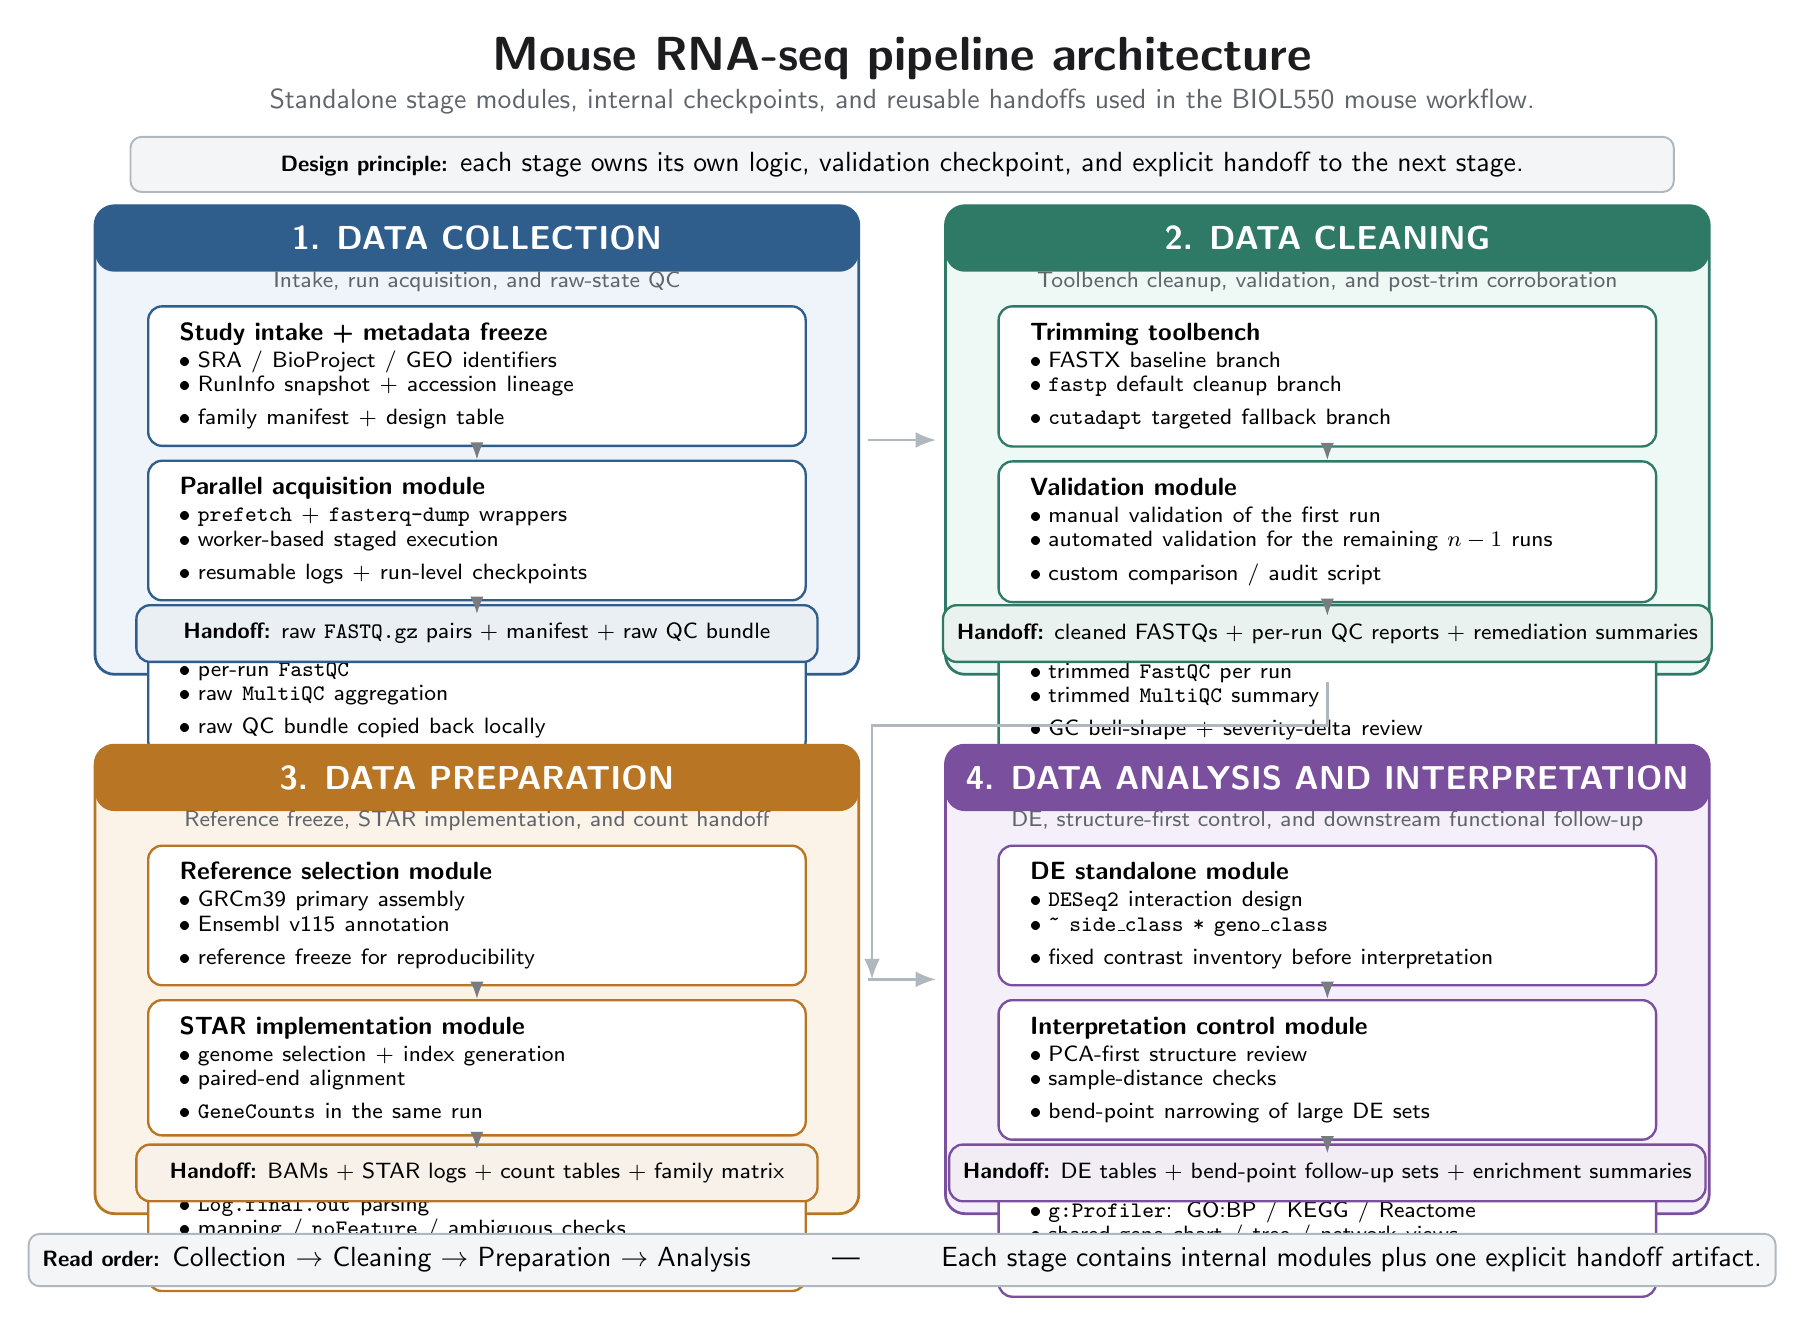
\begin{tikzpicture}[x=1cm,y=1cm]

% Title block
\node[font=\bfseries\fontsize{18}{20}\selectfont, text=ink] at (10.6,15.7) {Mouse RNA-seq pipeline architecture};
\node[font=\fontsize{9.7}{10.8}\selectfont, text=muted, align=center] at (10.6,15.15)
{Standalone stage modules, internal checkpoints, and reusable handoffs used in the BIOL550 mouse workflow.};
\node[topnote, minimum width=19.6cm, minimum height=0.7cm] at (10.6,14.35)
{{\bfseries\fontsize{8.2}{9.1}\selectfont Design principle:} each stage owns its own logic, validation checkpoint, and explicit handoff to the next stage.};

% Geometry
\def\stageW{9.7}
\def\stageH{5.95}
\def\modW{8.35}
\def\modH{1.05}
\def\modGap{0.16}
\def\headOffset{0.43}

% ----- Stage 1 -----
\node[stageframe, draw=collect, fill=collectbg, minimum width=\stageW cm, minimum height=\stageH cm] (S1) at (5.2,10.85) {};
\node[stagehead, fill=collect, minimum width=\stageW cm] at ($(S1.north)+(0,-\headOffset)$) {1. DATA COLLECTION};
\node[font=\fontsize{8.0}{8.9}\selectfont, text=muted, align=center] at ($(S1.north)+(0,-0.98)$) {Intake, run acquisition, and raw-state QC};
\node[module, draw=collect, minimum width=\modW cm, text width=7.55cm, minimum height=\modH cm, anchor=north] (s1a) at ($(S1.north)+(0,-1.28)$) {\modtitle{Study intake + metadata freeze}\\[1pt]
\modbody{\bul SRA / BioProject / GEO identifiers\\
\bul RunInfo snapshot + accession lineage\\
\bul family manifest + design table}};
\node[module, draw=collect, minimum width=\modW cm, text width=7.55cm, minimum height=\modH cm, anchor=north] (s1b) at ($(s1a.south)+(0,-\modGap)$) {\modtitle{Parallel acquisition module}\\[1pt]
\modbody{\bul \texttt{prefetch} + \texttt{fasterq-dump} wrappers\\
\bul worker-based staged execution\\
\bul resumable logs + run-level checkpoints}};
\node[module, draw=collect, minimum width=\modW cm, text width=7.55cm, minimum height=\modH cm, anchor=north] (s1c) at ($(s1b.south)+(0,-\modGap)$) {\modtitle{Raw QC module}\\[1pt]
\modbody{\bul per-run \texttt{FastQC}\\
\bul raw \texttt{MultiQC} aggregation\\
\bul raw QC bundle copied back locally}};
\node[handoff, draw=collect, fill=collect!10, minimum width=8.65cm, minimum height=0.72cm, anchor=south] at ($(S1.south)+(0,0.16)$)
{\textbf{Handoff:} raw \texttt{FASTQ.gz} pairs + manifest + raw QC bundle};

% ----- Stage 2 -----
\node[stageframe, draw=clean, fill=cleanbg, minimum width=\stageW cm, minimum height=\stageH cm] (S2) at (16.0,10.85) {};
\node[stagehead, fill=clean, minimum width=\stageW cm] at ($(S2.north)+(0,-\headOffset)$) {2. DATA CLEANING};
\node[font=\fontsize{8.0}{8.9}\selectfont, text=muted, align=center] at ($(S2.north)+(0,-0.98)$) {Toolbench cleanup, validation, and post-trim corroboration};
\node[module, draw=clean, minimum width=\modW cm, text width=7.55cm, minimum height=\modH cm, anchor=north] (s2a) at ($(S2.north)+(0,-1.28)$) {\modtitle{Trimming toolbench}\\[1pt]
\modbody{\bul FASTX baseline branch\\
\bul \texttt{fastp} default cleanup branch\\
\bul \texttt{cutadapt} targeted fallback branch}};
\node[module, draw=clean, minimum width=\modW cm, text width=7.55cm, minimum height=\modH cm, anchor=north] (s2b) at ($(s2a.south)+(0,-\modGap)$) {\modtitle{Validation module}\\[1pt]
\modbody{\bul manual validation of the first run\\
\bul automated validation for the remaining \(n-1\) runs\\
\bul custom comparison / audit script}};
\node[module, draw=clean, minimum width=\modW cm, text width=7.55cm, minimum height=\modH cm, anchor=north] (s2c) at ($(s2b.south)+(0,-\modGap)$) {\modtitle{Post-trim QC corroboration}\\[1pt]
\modbody{\bul trimmed \texttt{FastQC} per run\\
\bul trimmed \texttt{MultiQC} summary\\
\bul GC bell-shape + severity-delta review}};
\node[handoff, draw=clean, fill=clean!10, minimum width=8.65cm, minimum height=0.72cm, anchor=south] at ($(S2.south)+(0,0.16)$)
{\textbf{Handoff:} cleaned FASTQs + per-run QC reports + remediation summaries};

% ----- Stage 3 -----
\node[stageframe, draw=prep, fill=prepbg, minimum width=\stageW cm, minimum height=\stageH cm] (S3) at (5.2,4.0) {};
\node[stagehead, fill=prep, minimum width=\stageW cm] at ($(S3.north)+(0,-\headOffset)$) {3. DATA PREPARATION};
\node[font=\fontsize{8.0}{8.9}\selectfont, text=muted, align=center] at ($(S3.north)+(0,-0.98)$) {Reference freeze, STAR implementation, and count handoff};
\node[module, draw=prep, minimum width=\modW cm, text width=7.55cm, minimum height=\modH cm, anchor=north] (s3a) at ($(S3.north)+(0,-1.28)$) {\modtitle{Reference selection module}\\[1pt]
\modbody{\bul GRCm39 primary assembly\\
\bul Ensembl v115 annotation\\
\bul reference freeze for reproducibility}};
\node[module, draw=prep, minimum width=\modW cm, text width=7.55cm, minimum height=\modH cm, anchor=north] (s3b) at ($(s3a.south)+(0,-\modGap)$) {\modtitle{STAR implementation module}\\[1pt]
\modbody{\bul genome selection + index generation\\
\bul paired-end alignment\\
\bul \texttt{GeneCounts} in the same run}};
\node[module, draw=prep, minimum width=\modW cm, text width=7.55cm, minimum height=\modH cm, anchor=north] (s3c) at ($(s3b.south)+(0,-\modGap)$) {\modtitle{Alignment review + count handoff}\\[1pt]
\modbody{\bul \texttt{Log.final.out} parsing\\
\bul mapping / \texttt{noFeature} / ambiguous checks\\
\bul reverse-stranded count matrix (column 4)}};
\node[handoff, draw=prep, fill=prep!10, minimum width=8.65cm, minimum height=0.72cm, anchor=south] at ($(S3.south)+(0,0.16)$)
{\textbf{Handoff:} BAMs + STAR logs + count tables + family matrix};

% ----- Stage 4 -----
\node[stageframe, draw=analysis, fill=analysisbg, minimum width=\stageW cm, minimum height=\stageH cm] (S4) at (16.0,4.0) {};
\node[stagehead, fill=analysis, minimum width=\stageW cm] at ($(S4.north)+(0,-\headOffset)$) {4. DATA ANALYSIS AND INTERPRETATION};
\node[font=\fontsize{8.0}{8.9}\selectfont, text=muted, align=center] at ($(S4.north)+(0,-0.98)$) {DE, structure-first control, and downstream functional follow-up};
\node[module, draw=analysis, minimum width=\modW cm, text width=7.55cm, minimum height=\modH cm, anchor=north] (s4a) at ($(S4.north)+(0,-1.28)$) {\modtitle{DE standalone module}\\[1pt]
\modbody{\bul \texttt{DESeq2} interaction design\\
\bul \texttt{\textasciitilde{} side\_class * geno\_class}\\
\bul fixed contrast inventory before interpretation}};
\node[module, draw=analysis, minimum width=\modW cm, text width=7.55cm, minimum height=\modH cm, anchor=north] (s4b) at ($(s4a.south)+(0,-\modGap)$) {\modtitle{Interpretation control module}\\[1pt]
\modbody{\bul PCA-first structure review\\
\bul sample-distance checks\\
\bul bend-point narrowing of large DE sets}};
\node[module, draw=analysis, minimum width=\modW cm, text width=7.55cm, minimum height=\modH cm, anchor=north] (s4c) at ($(s4b.south)+(0,-\modGap)$) {\modtitle{GO / follow-up module}\\[1pt]
\modbody{\bul \texttt{g:Profiler}: GO:BP / KEGG / Reactome\\
\bul shared-gene chart / tree / network views\\
\bul anchor genes + report / paper figures}};
\node[handoff, draw=analysis, fill=analysis!10, minimum width=8.65cm, minimum height=0.72cm, anchor=south] at ($(S4.south)+(0,0.16)$)
{\textbf{Handoff:} DE tables + bend-point follow-up sets + enrichment summaries};

% internal arrows
\draw[vflow] (s1a.south) -- (s1b.north);
\draw[vflow] (s1b.south) -- (s1c.north);
\draw[vflow] (s2a.south) -- (s2b.north);
\draw[vflow] (s2b.south) -- (s2c.north);
\draw[vflow] (s3a.south) -- (s3b.north);
\draw[vflow] (s3b.south) -- (s3c.north);
\draw[vflow] (s4a.south) -- (s4b.north);
\draw[vflow] (s4b.south) -- (s4c.north);

% stage arrows: snake layout
\draw[flow] ($(S1.east)+(0.10,0)$) -- ($(S2.west)+(-0.10,0)$);
\draw[flow] ($(S2.south)+(0,-0.08)$) -- ++(0,-0.55) -| ($(S3.east)+(0.15,0)$);
\draw[flow] ($(S3.east)+(0.10,0)$) -- ($(S4.west)+(-0.10,0)$);

% compact legend
\node[topnote, minimum width=19.6cm, minimum height=0.62cm, anchor=north] at (10.6,0.78)
{{\bfseries\fontsize{8.1}{9}\selectfont Read order:} Collection $\rightarrow$ Cleaning $\rightarrow$ Preparation $\rightarrow$ Analysis \hspace{0.8cm} | \hspace{0.8cm} Each stage contains internal modules plus one explicit handoff artifact.};

\end{tikzpicture}
\end{document}
